
\de{ĐỀ THI GIỮA HỌC KỲ I NĂM HỌC 2023-2024}{THPT Võ Văn Kiệt}

%Câu 1...........................
\begin{bt}%[0D1H1-4]%[Dự án đề kiểm tra Toán 10 GHKI NH23-24 - Đặng Tân Hoài]%[THPT VÕ VĂN KIỆT - Tp Hồ Chí Minh]
	Cho mệnh đề: \lq\lq Nếu tứ giác $ABCD$ là hình chữ nhật có hai đường chéo vuông góc thì nó là hình vuông\rq\rq . Hãy phát biểu mệnh đề trên bằng cách sử dụng khái niệm \lq\lq điều kiện đủ\rq\rq .
	\loigiai{
		Tứ giác $ABCD$ là hình chữ nhật có hai đường chéo vuông góc là \textbf{điều kiện đủ} để nó là hình vuông.
	}
\end{bt}

%Câu 2...........................
\begin{bt}%[0D1H1-5]%[Dự án đề kiểm tra Toán 10 GHKI NH23-24 - Đặng Tân Hoài]%[THPT VÕ VĂN KIỆT - Tp Hồ Chí Minh]
	Phát biểu mệnh đề phủ định của mệnh đề $A\colon$ \lq\lq $\forall x \in \mathbb{R},~x^2-4x+4\ge 0$\rq\rq.
	\loigiai{
		Ta có $\overline{A}\colon$ \lq\lq $\exists x \in \mathbb{R},~x^2-4x+4< 0$\rq\rq.\\
		Phát biểu: \lq\lq Tồn tại số thực $x$ thỏa mãn bất phương trình $x^2-4x+4< 0$\rq\rq.
	}
\end{bt}

%Câu 3...........................
\begin{bt}%[0D1N3-1]%[Dự án đề kiểm tra Toán 10 GHKI NH23-24 - Đặng Tân Hoài]%[THPT VÕ VĂN KIỆT - Tp Hồ Chí Minh]
	Cho hai tập $A=\{-3;-1;0;2;4\}$ và $B=\{1;2;3;4\}$. Xác định $A\cap B$.
	\loigiai{
	Ta có	$A\cap B=\{2;4\}$.
	}
\end{bt}

%Câu 4...........................
\begin{bt}%[0D1H2-3]%[Dự án đề kiểm tra Toán 10 GHKI NH23-24 - Đặng Tân Hoài]%[THPT VÕ VĂN KIỆT - Tp Hồ Chí Minh]
	Hãy viết lại tập hợp sau bằng cách dùng các ký hiệu khoảng, đoạn, nửa khoảng
	$$H=\left\lbrace x\in \mathbb{R}\,\mid\, x+9>3-x \text{ và } 2x>3x-10 \right\rbrace.$$
	\loigiai{
		Ta có $\heva{& x+9>3-x\\& 2x>3x-10} \Leftrightarrow \heva{& x>-3\\& x<10} \Leftrightarrow -3<x<10$.
		\immini{
			Mà $x\in \mathbb{R}$ nên $H=(-3;10)$.
		}{\vspace*{-0.5cm}
			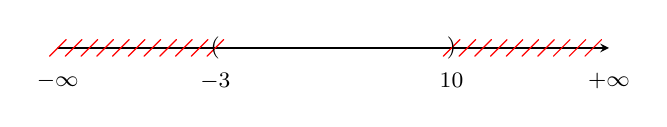
\begin{tikzpicture}[font=\footnotesize, line join=round, line cap=round, >=stealth]
				\tikzset{giao/.pic={
						\draw[->](0,0)--(7,0);
						\foreach \i in{0,0.2,...,2.0,5.0,5.2,...,6.8}
						\draw[red](\i,0)--++(45:0.15)(\i,0)--++(-135:0.15);
						\path(2,0)node[scale=1]{$($}(5,0)node[scale=1]{$)$};
						\path(2,0)node[below=2mm]{$-3$}(5,0)node[below=2mm]{$10$};
						\path(0,0)node[below=2mm]{$-\infty$}(7,0)node[below=2mm]{$+\infty$};
				}}
				\path (0,0)pic{giao};
		\end{tikzpicture}	}
	}
\end{bt}

%Câu 5...........................
\begin{bt}%[0H4V1-2]%[Dự án đề kiểm tra Toán 10 GHKI NH23-24 - Đặng Tân Hoài]%[THPT VÕ VĂN KIỆT - Tp Hồ Chí Minh]
	Cho $\cos \alpha =\dfrac{12}{13}$ với $0^\circ <\alpha <90^\circ$. Tính $\sin \alpha$. 
	\loigiai{
		Ta có $\sin^2 \alpha + \cos^2 \alpha =1 \Rightarrow \sin^2 \alpha = 1- \cos^2 \alpha = 1-\left(\dfrac{12}{13}\right)^2 = \dfrac{25}{169} \Rightarrow \sin \alpha = \pm \dfrac{5}{13}$.\\
		Mà $0^\circ <\alpha <90^\circ$ nên $\sin \alpha = \dfrac{5}{13}$.
	}
\end{bt}

%Câu 6...........................
\begin{bt}%[0H4V1-3]%[Dự án đề kiểm tra Toán 10 GHKI NH23-24 - Đặng Tân Hoài]%[THPT VÕ VĂN KIỆT - Tp Hồ Chí Minh]
	Chứng minh rằng trong tam giác $ABC$ ta luôn có $\sin (A+C)=\sin B$.
	\loigiai{
		Ta có $\widehat{A}+\widehat{B}+\widehat{C}=180^\circ \Leftrightarrow \left(\widehat{A}+\widehat{C}\right)+\widehat{B}=180^\circ$ nên hai góc $\widehat{A}+\widehat{C}$ và $\widehat{B}$ là góc bù nhau.\\
		Vậy $\sin (A+C)=\sin B$ (điều phải chứng minh).
	}
\end{bt}

%Câu 7...........................
\begin{bt}%[0H4H2-2]%[Dự án đề kiểm tra Toán 10 GHKI NH23-24 - Đặng Tân Hoài]%[THPT VÕ VĂN KIỆT - Tp Hồ Chí Minh]
	Cho tam giác $ABC$ có $a=8$, $b=6$, $\widehat{C}=150^\circ$. Tính diện tích tam giác $ABC$.
	\loigiai{
		Diện tích tam giác $ABC$ là $S=\dfrac{1}{2}ab\sin C = \dfrac{1}{2}\cdot 8 \cdot 6 \cdot \sin 150^\circ=12$
	}
\end{bt}

%Câu 8...........................
\begin{bt}%[0H4H2-1]%[Dự án đề kiểm tra Toán 10 GHKI NH23-24 - Đặng Tân Hoài]%[THPT VÕ VĂN KIỆT - Tp Hồ Chí Minh]
	Cho tam giác $ABC$ có $AB=5$, $BC=8$, $AC=6$. Tính $\cos A$.
	\loigiai{
		Áp dụng hệ quả định lý cô-sin vào tam giác $ABC$, ta có 
		$$\cos A = \dfrac{AB^2+AC^2-BC^2}{2\cdot AB \cdot AC}= \dfrac{5^2+6^2-8^2}{2\cdot 5 \cdot 6}=-\dfrac{1}{20}.$$
	}
\end{bt}

%Câu 2a...........................
\begin{bt}%[0D2H1-2]%[Dự án đề kiểm tra Toán 10 GHKI NH23-24 - Đỗ ĐƯờng Hiếu]%[THPT Võ Văn Kiệt- Tp HCM]
	Xác định miền nghiệm của bất phương trình bậc nhất hai ẩn $x+y-2\ge 0$.
	\loigiai{
		\immini{Vẽ đường thẳng $d\colon x+y-2=0$.\\
			Xét điểm $O(0;0)$, ta có $0+0-2<0$.\\
			Do đó miền nghiệm của bất phương trình là nửa mặt phẳng bờ $d$ (kể cả đường thẳng $d$) không chứa điểm $O$.}
		{\begin{tikzpicture}[scale=0.9,line join=round, line cap=round,>=stealth]
				%\tikzset{every node/.style={scale=0.9}}
				\begin{scope}
					\draw[->] (-1,0)--(3,0) node[below]{$x$};
					\draw[->] (0,-1)--(0,3) node[right]{$y$};
					\path (2,0)node[below]{$2$}
					(0,2)node[left]{$2$}	;
					\clip (-1,-1) rectangle (3,3);
					\fill[pattern=north east lines, opacity=60] (-1,3)--(3,3)--(3,-1)--cycle;
					\draw (-1,3)--(3,-1);					
					\draw (0,0) node[below left]{$O$};					
				\end{scope}	
		\end{tikzpicture}}	
	}
\end{bt}

%Câu 2b...........................
\begin{bt}%[0D1H2-3]%[Dự án đề kiểm tra Toán 10 GHKI NH23-24 - Đỗ ĐƯờng Hiếu]%[THPT Võ Văn Kiệt- Tp HCM]
	Tìm tập xác định của hàm số $y=\sqrt{x-1}+\dfrac{1}{x-2}$.
	\loigiai{
		Hàm số $y=\sqrt{x-1}+\dfrac{1}{x-2}$ xác định khi và chỉ khi $\heva{&x-1>0\\&x-2\ne 0}\Leftarrow 1<x\ne 2$.\\
		Vậy tập xác định của hàm số là $\mathscr{D}=(1;+\infty)\setminus\{2\}$.
	}
\end{bt}

%Câu 2c...........................
\begin{bt}%[0H4H1-3]%[Dự án đề kiểm tra Toán 10 GHKI NH23-24 - Đỗ ĐƯờng Hiếu]%[THPT Võ Văn Kiệt- Tp HCM]
	Đơn giản các biểu thức $A=\sin 110^\circ-\sin 70^\circ+\cos 160^\circ+\cos 20^\circ-23\tan 12^\circ\cdot \cot 168^\circ+2000$.
	\loigiai{
		Ta có
		\begin{eqnarray*}
			A&=&\sin (180^\circ-70^\circ)-\sin 70^\circ+\cos (180^\circ-20^\circ)+\cos 20^\circ+\\
			&&-23\cdot \tan 12^\circ\cdot \cot(180^\circ-12^\circ)+2000\\
			&=&\sin 70^\circ-\sin 70^\circ-\cos20^\circ+\cos 20^\circ+23\cdot \tan 12^\circ\cdot \cot 12^\circ+2000=2023.	
		\end{eqnarray*}
	}
\end{bt}

%Câu 2d...........................
\begin{bt}%[0H4H2-1]%[Dự án đề kiểm tra Toán 10 GHKI NH23-24 - Đỗ ĐƯờng Hiếu]%[THPT Võ Văn Kiệt- Tp HCM]
	Cho tam giác $ABC$ thỏa $2ab(\cos C-1)+c^2=0$. Chứng minh tam giác $ABC$ cân.
	\loigiai{
		Ta có \vspace*{-0.5 cm}
		\begin{eqnarray*}
			&&2ab(\cos C-1)+c^2=0\\
			&\Leftrightarrow& 2ab\cos C-2ab+a^2+b^2-2ab\cos C=0\\
			&\Leftrightarrow& (a-b)^2=0\\
			&\Leftrightarrow& a=b.
		\end{eqnarray*}
		Suy ra tam giác $ABC$ cân đỉnh $C$.
	}
\end{bt}

%Câu 3...........................
\begin{bt}%[0D1V3-5]%[Dự án đề kiểm tra Toán 10 GHKI NH23-24 - Nguyễn Văn Sang]%[THPT Võ Văn Kiệt - Tp HCM]
	Trong một hoạt động thể thao tổ chức tại hội trại, lớp $10A$ có $15$ học sinh đăng ký chơi môn đá cầu, $20$ học sinh đăng ký chơi môn cầu lông. Tìm số học sinh đăng ký chơi cả hai môn biết $10A$ có $40$ học sinh và có $10$ học sinh không đăng ký chơi cả hai môn đá cầu và cầu lông.
	\loigiai{
		\begin{itemize}
			\item Gọi $A$ là tập hợp số học sinh đăng ký chơi đá cầu suy ra $n(A)=15$.
			\item Gọi $B$ là tập hợp số học sinh đăng ký chơi cầu lông suy ra $n(B)=20$.
			\item Gọi $C=A\cup B$ là tập hợp số học sinh đăng ký chơi ít nhất một trong hai môn đá cầu hoặc cầu lông.
			\item Gọi $D=A\cap B$ là tập hợp số học sinh đăng ký chơi cả hai môn đá cầu và cầu lông.
		\end{itemize}
		Do có $10$ học sinh không đăng ký chơi môn nào, tức là có $40-10=30$ học sinh đăng ký chơi ít nhất một trong hai môn (đá cầu hoặc cầu lông) suy ra $n(C)=30$.\\
		Ta được $n(D)=n(A)+n(B)-n(C)=15+20-30=5$.\\
		Vậy có $5$ học sinh lớp $10A$ đăng ký chơi cả hai môn đá cầu và cầu lông.
	}
\end{bt}
%%Câu 3:
\begin{bt}%[0H4V3-2]%[Dự án đề kiểm tra Toán 10 GHKI NH23-24 - Nguyễn Văn Sang]%[THPT Võ Văn Kiệt - Tp HCM]
	\immini
	{
		Hai chiếc tàu thuỷ $P$ và $Q$ cách nhau $300$ m và thẳng hàng với chân $B$ của tháp hải đăng $AB$ ở trên bờ biển. Từ $P$ và $Q$, người ta nhìn thấy tháp hải đăng $AB$ dưới các góc $\widehat{BPA}=35^{\circ}$ và $\widehat{BQA}=48^{\circ}$. Tính chiều cao của tháp hải đăng đó.
	}
	{
		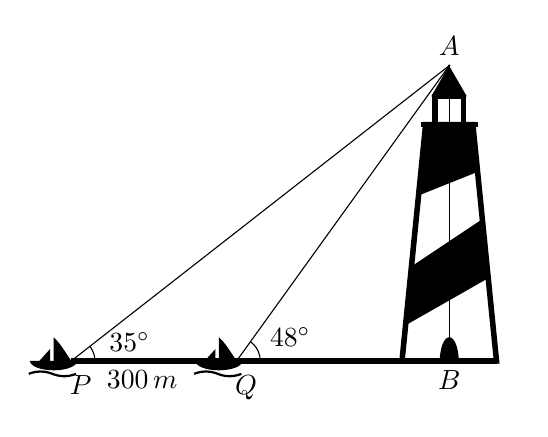
\begin{tikzpicture}[scale=.3]
			\draw [line width=2pt] (0,0)--(1,10)--(3,10)--(4,0)--cycle;
			\fill (3,10)--(3.2,8)--(0.7,7)--(1,10)--cycle;
			\fill (0.14,1.5)--(0.4,4)--(3.4,6)--(3.65,3.5)--cycle;
			\fill (2.4,0) arc(0:180:0.4 cm and 1 cm);
			\draw[line width=2pt] (4,0)--(-14,0);
			\draw[line width=2pt] (0.8,10)--(3.2,10);
			\draw[line width=2pt] (1.4,10)--++(90:1.2)--++(0:1.2)--++(-90:1.2);
			\fill (1.24,11.2)--++(0:1.5)--++(120:1.5)--cycle;
			\begin{scope}
				\draw (-14,0)--(2,12.5);
				\clip (2,12.5) -- (-14,0) -- (5,0);
				\draw (-14,0) circle (1cm);
				\draw (-13+0.2,0) node[above right]{$35^\circ$};
			\end{scope}
			\begin{scope}
				\draw (-7,0)--(2,12.5);
				\clip (2,12.5) -- (-7,0) -- (5,0);
				\draw (-7,0) circle (1cm);
				\draw (-6,0.2) node[above right]{$48^\circ$};
			\end{scope}
			\draw (2,0)--(2,12.5);
			\draw (-11,0) node[below]{$300\,m$};
			\fill (2,12.5) circle (1.5pt) node[above]{$A$};
			\fill (2,0) circle (1.5pt) node[below]{$B$};
			\draw (-14+0.4,0-0.2) node[below]{$P$};
			\draw (-7+0.4,0-0.2)  node[below]{$Q$};
			\fill (-13.75,0) arc(0:-180:1 cm and 0.4 cm);
			\fill (-14,0)..controls(-14.5,0.75)..(-14.75,1)--(-14.75,0);
			\fill (-15.35,0)--(-15+0.1,0.5)--(-15+0.1,0)--cycle;
			\draw[thick] (-15.5-0.3,-0.75+0.2) parabola bend (-15.5+0.5-0.3,-0.75+0.1+0.2) (-15+0.5-0.3,-0.75+0.2) parabola bend (-14.5+0.5-0.3,-0.75-0.1+0.2) (-14+0.5-0.3,-0.75+0.2);
			\fill (-6.75,0) arc(0:-180:1 cm and 0.4 cm);
			\fill (-7,0)..controls(-7.5,0.75)..(-7.75,1)--(-7.75,0);
			\fill (-8.35,0)--(-8+0.1,0.5)--(-8+0.1,0)--cycle;	
			\draw[thick] (-8.5-0.3,-0.75+0.2) parabola bend (-8.5+0.5-0.3,-0.75+0.1+0.2) (-8+0.5-0.3,-0.75+0.2) parabola bend (-7.5+0.5-0.3,-0.75-0.1+0.2) (-7+0.5-0.3,-0.75+0.2);
			%%hình được vẽ bởi %%sang nguyễn văn
		\end{tikzpicture}
	}
	\loigiai{
		\immini
		{
			Trong tam giác $\triangle APQ$, ta có $\widehat{PQA}=180^\circ-48^\circ=132^\circ$ và $\widehat{PAQ}=180^\circ-132^\circ-35^\circ=13^\circ$.\\
			Áp dụng định lý sin trong tam giác $\triangle APQ$, ta được $$\dfrac{AP}{\sin\widehat{PQA}}=\dfrac{PQ}{\sin\widehat{PAQ}}\Leftrightarrow AP=\dfrac{PQ\cdot\sin\widehat{PQA}}{\sin\widehat{PAQ}} \Leftrightarrow AP=\dfrac{300\cdot \sin{132^\circ}}{\sin{13^\circ}}.$$
			Trong tam giác $\triangle ABP$, ta có
			$$AB=AP\cdot\sin\widehat{APQ}=\dfrac{300\cdot \sin{132^\circ}}{\sin{13^\circ}}\cdot\sin{35^\circ}\approx 568{,}46\,\text{m.}$$
			Vậy chiều cao của tháp hải đăng là $h\approx 568{,}46$ m.
		}
		{
			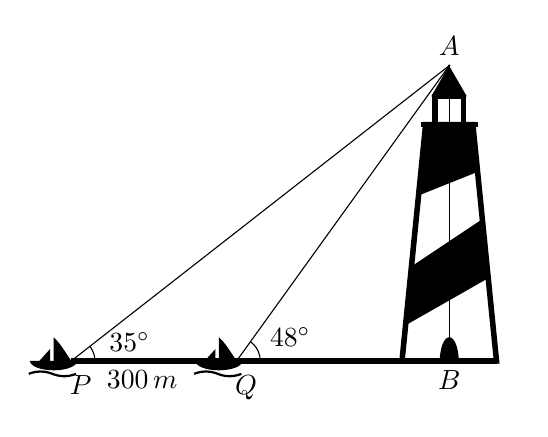
\begin{tikzpicture}[scale=.3]
				\draw [line width=2pt] (0,0)--(1,10)--(3,10)--(4,0)--cycle;
				\fill (3,10)--(3.2,8)--(0.7,7)--(1,10)--cycle;
				\fill (0.14,1.5)--(0.4,4)--(3.4,6)--(3.65,3.5)--cycle;
				\fill (2.4,0) arc(0:180:0.4 cm and 1 cm);
				\draw[line width=2pt] (4,0)--(-14,0);
				\draw[line width=2pt] (0.8,10)--(3.2,10);
				\draw[line width=2pt] (1.4,10)--++(90:1.2)--++(0:1.2)--++(-90:1.2);
				\fill (1.24,11.2)--++(0:1.5)--++(120:1.5)--cycle;
				\begin{scope}
					\draw (-14,0)--(2,12.5);
					\clip (2,12.5) -- (-14,0) -- (5,0);
					\draw (-14,0) circle (1cm);
					\draw (-13+0.2,0) node[above right]{$35^\circ$};
				\end{scope}
				\begin{scope}
					\draw (-7,0)--(2,12.5);
					\clip (2,12.5) -- (-7,0) -- (5,0);
					\draw (-7,0) circle (1cm);
					\draw (-6,0.2) node[above right]{$48^\circ$};
				\end{scope}
				\draw (2,0)--(2,12.5);
				\draw (-11,0) node[below]{$300\,m$};
				\fill (2,12.5) circle (1.5pt) node[above]{$A$};
				\fill (2,0) circle (1.5pt) node[below]{$B$};
				\draw (-14+0.4,0-0.2) node[below]{$P$};
				\draw (-7+0.4,0-0.2)  node[below]{$Q$};
				\fill (-13.75,0) arc(0:-180:1 cm and 0.4 cm);
				\fill (-14,0)..controls(-14.5,0.75)..(-14.75,1)--(-14.75,0);
				\fill (-15.35,0)--(-15+0.1,0.5)--(-15+0.1,0)--cycle;
				\draw[thick] (-15.5-0.3,-0.75+0.2) parabola bend (-15.5+0.5-0.3,-0.75+0.1+0.2) (-15+0.5-0.3,-0.75+0.2) parabola bend (-14.5+0.5-0.3,-0.75-0.1+0.2) (-14+0.5-0.3,-0.75+0.2);
				\fill (-6.75,0) arc(0:-180:1 cm and 0.4 cm);
				\fill (-7,0)..controls(-7.5,0.75)..(-7.75,1)--(-7.75,0);
				\fill (-8.35,0)--(-8+0.1,0.5)--(-8+0.1,0)--cycle;	
				\draw[thick] (-8.5-0.3,-0.75+0.2) parabola bend (-8.5+0.5-0.3,-0.75+0.1+0.2) (-8+0.5-0.3,-0.75+0.2) parabola bend (-7.5+0.5-0.3,-0.75-0.1+0.2) (-7+0.5-0.3,-0.75+0.2);
				%%hình được vẽ bởi %%sang nguyễn văn
			\end{tikzpicture}
		}
		
	}
\end{bt}

%Câu 4...........................
\begin{bt}%[0D3V2-2]%[Dự án đề kiểm tra Toán 10 GHKI NH23-24 - Nguyễn Văn Sang]%[THPT Võ Văn Kiệt - Tp HCM]
	Cho hàm số $f(x)= \heva{&\dfrac{2 \sqrt{x+2}-3}{x-1} & \text { khi } x \geq 2 \\& x^2+m^2-2 m & \text { khi } x<2}$ với $m$ là tham số thực.\\
	Đặt $A=f(1)+f(2)$, xác định $m$ để $A$ đạt giá trị nhỏ nhất.
	\loigiai{
		Ta có
		\begin{itemize}
			\item $f(1)=m^2-2m+1$.
			\item $f(2)=\dfrac{2 \sqrt{2+2}-3}{2-1}=1$.
			\item $A=f(1)+f(2)=m^2-2m+1+1=(m-1)^2+1\geq 1, \forall m\in \mathbb{R}$.\\
			Vậy giá trị nhỏ nhất của $A=1$ khi $m-1=0 \Leftrightarrow m=1$.
		\end{itemize}
	}
\end{bt}

\textbf{KHÔNG HỌC CHUYÊN ĐỀ}

\begin{bt}%[0H4V2-3]%[Dự án đề kiểm tra Toán 10 GHKI NH23-24 - Lê Hùng Thắng]%[THPT Võ Văn Kiệt - HCM]
	Cho tam giác $A B C$ với $B C=a, A C=b, A B=c$. Gọi $p$ là nửa chu vi của tam giác.
	Chứng minh rằng $a b c (\cos A+\cos B+\cos C)=a^2(p-a)+b^2(p-b)+c^2(p-c)$.
	\loigiai{
		Ta có $abc\cos A=abc\dfrac{b^2+c^2-a^2}{2bc}=\dfrac{a(b^2+c^2-a^2)}{2}$.\\
		Tương tự $abc \cos B=\dfrac{b(a^2+c^2-b^2)}{2}$;	$abc \cos C=\dfrac{c(a^2+b^2-c^2)}{2}$.\\
		Do đó $\begin{aligned}[t]
			&\, a b c (\cos A+\cos B+\cos C) \\
			= &\, \dfrac{a(b^2+c^2-a^2)}{2}+ \dfrac{b(a^2+c^2-b^2)}{2}+\dfrac{c(a^2+b^2-c^2)}{2}\\
			= &\, \dfrac{a^2(b+c-a)}{2}+ \dfrac{b^2(a+c-b)}{2}+\dfrac{c^2(a+b-c)}{2}\\
			= &\, a^2(p-a)+b^2(p-b)+c^2(p-c). 
		\end{aligned}$\\
Suy ra điều phải chứng minh.
		}
\end{bt}

\textbf{CÓ HỌC CHUYÊN ĐỀ}
\begin{bt}%[0H4C2-4]%[Dự án đề kiểm tra Toán 10 GHKI NH23-24 - Lê Hùng Thắng]%[THPT Võ Văn Kiệt - HCM]
	Cho tam giác $A B C$, với các đường cao $h_a, h_b, h_c$ và bán kính đường tròn nội tiếp $r$ của tam giác $A B C$ thỏa mãn $h_a+h_b+h_c=9 r$. Chứng minh tam giác $A B C$ là tam giác đều.
	\loigiai{Ta có $S=\dfrac{1}{2}a\cdot h_a=\dfrac{1}{2}b\cdot h_b=\dfrac{1}{2}c\cdot h_c \Rightarrow h_a+h_b+h_c=2S\left(\dfrac{1}{a}+\dfrac{1}{b}+\dfrac{1}{c}\right)$.\\
		Lại có $S=pr \Rightarrow r=\dfrac{S}{p}=\dfrac{2S}{a+b+c}$.\\
		Theo đề
		\allowdisplaybreaks \vspace*{-0.7cm}
		\begin{eqnarray*} 
			& & h_a+h_b+h_c=9 r \\
			& \Leftrightarrow & 2S\left(\dfrac{1}{a}+\dfrac{1}{b}+\dfrac{1}{c}\right) =9\cdot \dfrac{2S}{a+b+c}\\
			& \Leftrightarrow & \left(\dfrac{1}{a}+\dfrac{1}{b}+\dfrac{1}{c}\right)(a+b+c)=9.
		\end{eqnarray*}
		Theo bất đẳng thức Cô-si ta có $\left(\dfrac{1}{a}+\dfrac{1}{b}+\dfrac{1}{c}\right)(a+b+c)\ge 9$.\\
		Dấu bằng xảy ra khi $a=b=c$ do đó tam giác $ABC$ là tam giác đều.}
\end{bt}



